%
% ---------------------------------------------------------------
% Copyright (C) 2012-2018 Gang Li
% ---------------------------------------------------------------
%
% This work is the default powerdot-tuliplab style test file and may be
% distributed and/or modified under the conditions of the LaTeX Project Public
% License, either version 1.3 of this license or (at your option) any later
% version. The latest version of this license is in
% http://www.latex-project.org/lppl.txt and version 1.3 or later is part of all
% distributions of LaTeX version 2003/12/01 or later.
%
% This work has the LPPL maintenance status "maintained".
%
% This Current Maintainer of this work is Gang Li.
%
%

\documentclass[
 size=14pt,
 paper=smartboard,  %a4paper, smartboard, screen
 mode=present, 		%present, handout, print
 display=slides, 	% slidesnotes, notes, slides
 style=tuliplab,  	% TULIP Lab style
 pauseslide,
 fleqn,leqno]{powerdot}


\usepackage{cancel}
\usepackage{caption}
\usepackage{stackengine}
\usepackage{smartdiagram}
\usepackage{attrib}
\usepackage{amssymb}
\usepackage{amsmath} 
\usepackage{amsthm} 
\usepackage{mathtools}
\usepackage{rotating}
\usepackage{graphicx}
\usepackage{boxedminipage}
\usepackage{rotate}
\usepackage{calc}
\usepackage[absolute]{textpos}
\usepackage{psfrag,overpic}
\usepackage{fouriernc}
\usepackage{pstricks,pst-3d,pst-grad,pstricks-add,pst-text,pst-node,pst-tree}
\usepackage{moreverb,epsfig,subfigure}
\usepackage{color}
\usepackage{booktabs}
\usepackage{etex}
\usepackage{breqn}
\usepackage{multirow}
\usepackage{natbib}
\usepackage{bibentry}
\usepackage{gitinfo2}
\usepackage{siunitx}
\usepackage{nicefrac}
%\usepackage{geometry}
%\geometry{verbose,letterpaper}
\usepackage{media9}
\usepackage{animate}
%\usepackage{movie15}
\usepackage{auto-pst-pdf}

\usepackage{breakurl}
\usepackage{fontawesome}
\usepackage{xcolor}
\usepackage{multicol}



\usepackage{verbatim}
\usepackage[utf8]{inputenc}
\usepackage{dtk-logos}
\usepackage{tikz}
\usepackage{adigraph}
%\usepackage{tkz-graph}
\usepackage{hyperref}
%\usepackage{ulem}
\usepackage{pgfplots}
\usepackage{verbatim}
\usepackage{fontawesome}


\usepackage{todonotes}
% \usepackage{pst-rel-points}
\usepackage{animate}
\usepackage{fontawesome}

\usepackage{listings}
\lstset{frameround=fttt,
frame=trBL,
stringstyle=\ttfamily,
backgroundcolor=\color{yellow!20},
basicstyle=\footnotesize\ttfamily}
\lstnewenvironment{code}{
\lstset{frame=single,escapeinside=`',
backgroundcolor=\color{yellow!20},
basicstyle=\footnotesize\ttfamily}
}{}


\usepackage{hyperref}
\hypersetup{ % TODO: PDF meta Data
  pdftitle={Presentation Title},
  pdfauthor={Gang Li},
  pdfpagemode={FullScreen},
  pdfborder={0 0 0}
}


% \usepackage{auto-pst-pdf}
% package to show source code

\definecolor{LightGray}{rgb}{0.9,0.9,0.9}
\newlength{\pixel}\setlength\pixel{0.000714285714\slidewidth}
\setlength{\TPHorizModule}{\slidewidth}
\setlength{\TPVertModule}{\slideheight}
\newcommand\highlight[1]{\fbox{#1}}
\newcommand\icite[1]{{\footnotesize [#1]}}

\newcommand\twotonebox[2]{\fcolorbox{pdcolor2}{pdcolor2}
{#1\vphantom{#2}}\fcolorbox{pdcolor2}{white}{#2\vphantom{#1}}}
\newcommand\twotoneboxo[2]{\fcolorbox{pdcolor2}{pdcolor2}
{#1}\fcolorbox{pdcolor2}{white}{#2}}
\newcommand\vpspace[1]{\vphantom{\vspace{#1}}}
\newcommand\hpspace[1]{\hphantom{\hspace{#1}}}
\newcommand\COMMENT[1]{}

\newcommand\placepos[3]{\hbox to\z@{\kern#1
        \raisebox{-#2}[\z@][\z@]{#3}\hss}\ignorespaces}

\renewcommand{\baselinestretch}{1.2}


\newcommand{\draftnote}[3]{
	\todo[author=#2,color=#1!30,size=\footnotesize]{\textsf{#3}}	}
% TODO: add yourself here:
%
\newcommand{\gangli}[1]{\draftnote{blue}{GLi:}{#1}}
\newcommand{\shaoni}[1]{\draftnote{green}{sn:}{#1}}
\newcommand{\gliMarker}
	{\todo[author=GLi,size=\tiny,inline,color=blue!40]
	{Gang Li has worked up to here.}}
\newcommand{\snMarker}
	{\todo[author=Sn,size=\tiny,inline,color=green!40]
	{Shaoni has worked up to here.}}

%%%%%%%%%%%%%%%%%%%%%%%%%%%%%%%%%%%%%%%%%%%%%%%%%%%%%%%%%%%%%%%%%%%%%%%%
% title
% TODO: Customize to your Own Title, Name, Address
%
\title{Bike Sharing Demand}
\author{
  Pratikshya Parajuli
  \\
  \\Ministry of Finance
  \\Governmnet of Nepal
  \\
}
%\date{\gitCommitterDate}


% Customize the setting of slides
\pdsetup{
% TODO: Customize the left footer, and right footer
rf=\href{http://www.tulip.org.au}{
Last Changed by: \textsc{\gitCommitterName}\ \gitVtagn-\gitAbbrevHash\ (\gitAuthorDate)
},
cf={Bike Sharing Demand},
}


\begin{document}

\maketitle

\begin{slide}[toc=,bm=]{Overview}
\tableofcontents[content=currentsection,type=1]
\end{slide}
%%
%%==========================================================================================

\section{Problem Definition}

\begin{slide}[toc=,bm=]{Bike Sharing Demand}
\begin{center}
\twotonebox{\rotatebox{90}{Defn}}{\parbox{.86\textwidth}
{Bike sharing demand aims to
forecast the use of the bikeshare system throughout the city. 
\begin{itemize}
\item Dataset comprises of the hourly rental data spanning two year having data fields such as  \textcolor{orange}{datetime}, {season}{temp} etc.
\item predict the \textcolor{orange}{total count} of bikes rented during each hour 
\end{itemize}
}}

\end{center}
\bigskip

%%==========================================================================================
%%==========================================================================================

\end{slide}
%%
%%==========================================================================================
\begin{slide}[toc=,bm=]{Data Summary}
  \begin{itemize}
    \item  Training Set provides the data and usage of the first 19 days of each month
    \item Test Set provides the data from the 20th to the end of the month
  \end{itemize}
  \bigskip
  \twocolumn[
\savevalue{lfrheight}=4.6cm,
\savevalue{lfrprop}={
linestyle=solid,framearc=.2,linewidth=1pt},
rfrheight=\usevalue{lfrheight},
rfrprop=\usevalue{lfrprop}
]{
  \begin{figure}
    \centering
    %\selectcolormodel{rgb}
    \centerline{\includegraphics[width=1.0\textwidth,height=0.4\textwidth]{graphics/img/Data_summary1.eps}}
  \end{figure}
  }{
  \begin{figure}
    %\centering
    %\selectcolormodel{rgb}
    \centerline{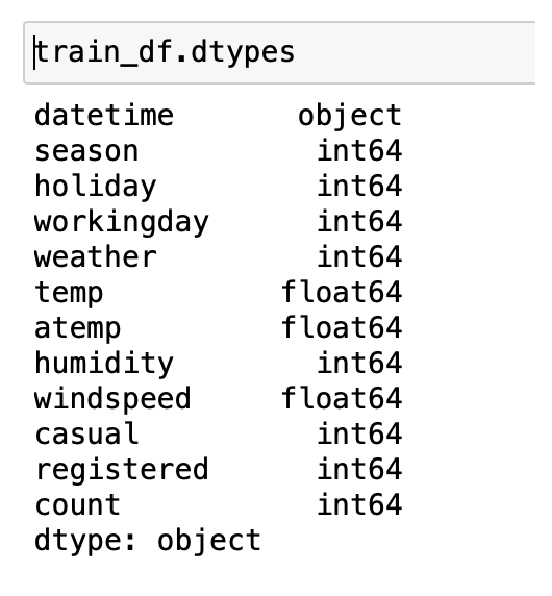
\includegraphics[width=0.5\textwidth,height=0.4\textwidth]{graphics/img/Data_summary2.eps}}
  \end{figure}
  }
  \begin{itemize}
   
     \item No missing values in the dataset
    
    \end{itemize}
  \bigskip
  
  \end{slide}
  %%
  %%==========================================================================================

\section{Exploratory Data Analysis}


%%==========================================================================================
%%
\begin{slide}[toc=,bm=]{Dataset Description}
  \begin{itemize}
     \item Data Fields
    \begin{itemize} 
      \item datetime - hourly date + timestamp
      \item season - 1 = spring, 2 = summer, 3 = fall, 4 = winter
      \item holiday - whether the day is considered a holiday
      \item workingday - whether the day is neither a weekend nor holiday
      \item weather - 1: Clear, Few clouds, Partly cloudy, Partly cloudy / 2: Mist + Cloudy, Mist + Broken clouds, Mist + Few clouds, Mist / 3: Light Snow, Light Rain + Thunderstorm + Scattered clouds, Light Rain + Scattered clouds / 4: Heavy Rain + Ice Pallets + Thunderstorm + Mist, Snow + Fog
      \item temp - temperature in Celsius
      \item atemp - "feels like" temperature in Celsius
      \item humidity - relative humidity
      \item windspeed - wind speed
      \item casual - number of non-registered user rentals initiated
      \item registered - number of registered user rentals initiated
      \item count - number of total rentals
    \end{itemize} 
    \end{itemize}

%%==========================================================================================

\end{slide}

\begin{slide}[toc=,bm=]{Data Preprocessing}

\begin{itemize}
\item Season, holiday, workingday, and weather are int type, but category type is more suitable, so convert to category type
\item split datetime into separate year, month, day, hour and dayofweek columns
\item Analyse the missing values
\item Remove datetime 

\end{itemize}
\end{slide}
%%
%%==========================================================================================

\begin{slide}[toc=,bm=]{Analysis of the features}

  \begin{itemize}
  \item \textcolor{orange}{Category Features} : Hour, weekday, month, Season, holiday, Workingday, weather 
  \item \textcolor{orange}{Numerical Features}:  temp, atemp, humidity, windspeed, registered and causal 
 
  \end{itemize}
  \end{slide}
  %%
  %%==========================================================================================

\begin{slide}[toc=,bm=]{ Outliers Analysis}

  \begin{itemize}
  \item From the Boxplot of count column, it is clearly visible that most of the data lies between 30-300 and a huge numbers of outliers are presesnt in the plot.
  \item Use the 3 sigma principle to remove outliers
  \end{itemize}
  \begin{figure}
    \centering
    %\selectcolormodel{rgb}
    \centerline{\includegraphics[scale=0.4,width=0.8\textwidth,height=0.4\textwidth]{graphics/img/countboxplot.eps}}
  \end{figure}
  \end{slide}
  %%
  %%==========================================================================================
  
  \begin{slide}[toc=,bm=]{ Data Visualization between count vs. month and season }

    \begin{itemize}
    \item The use of shared bicycles from November to April will be a little less than in other months, which may be due to seasonal reasons. 
    \end{itemize}
  
    \begin{figure}
      \centering
      %\selectcolormodel{rgb}
      \centerline{\includegraphics[scale=0.4,width=0.5\textwidth,height=0.4\textwidth]{graphics/img/data_vis1.eps}}
      \caption{Data Visualization between count vs. month and season}\label{fig:Data Visualization between count vs. month and season}
    \end{figure}
    \end{slide}
    %%
    %%==========================================================================================
    \begin{slide}[toc=,bm=]{ Data Visualization between count vs. weekdays and usertype }

      \begin{itemize}
      \item The use of shared bicycles in winter and spring is relatively small compared to summer and autumn, which is mutually confirmed with the conclusions generated in the above months.
      \end{itemize}
      Histogram Plot of Count
      \begin{figure}
        \centering
        %\selectcolormodel{rgb}
        \centerline{\includegraphics[scale=0.4,width=0.5\textwidth,height=0.4\textwidth]{graphics/img/data_vis2.eps}}
        \caption{Data Visualization between count vs. weekdays and usertype}\label{fig:Data Visualization between count vs. weekdays and usertype}
      \end{figure}
      \end{slide}
      %%
      %%==========================================================================================

      \begin{slide}[toc=,bm=]{ Data Visualization of count and [temp, windspeed, humidity]}

        \begin{itemize}
        \item From the scatter plot,  windspeed has many values of 0 and is separated from other values, so it is predicted that this is not an actual measured value.
        \end{itemize}
        \begin{figure}
          \centering
          %\selectcolormodel{rgb}
          \centerline{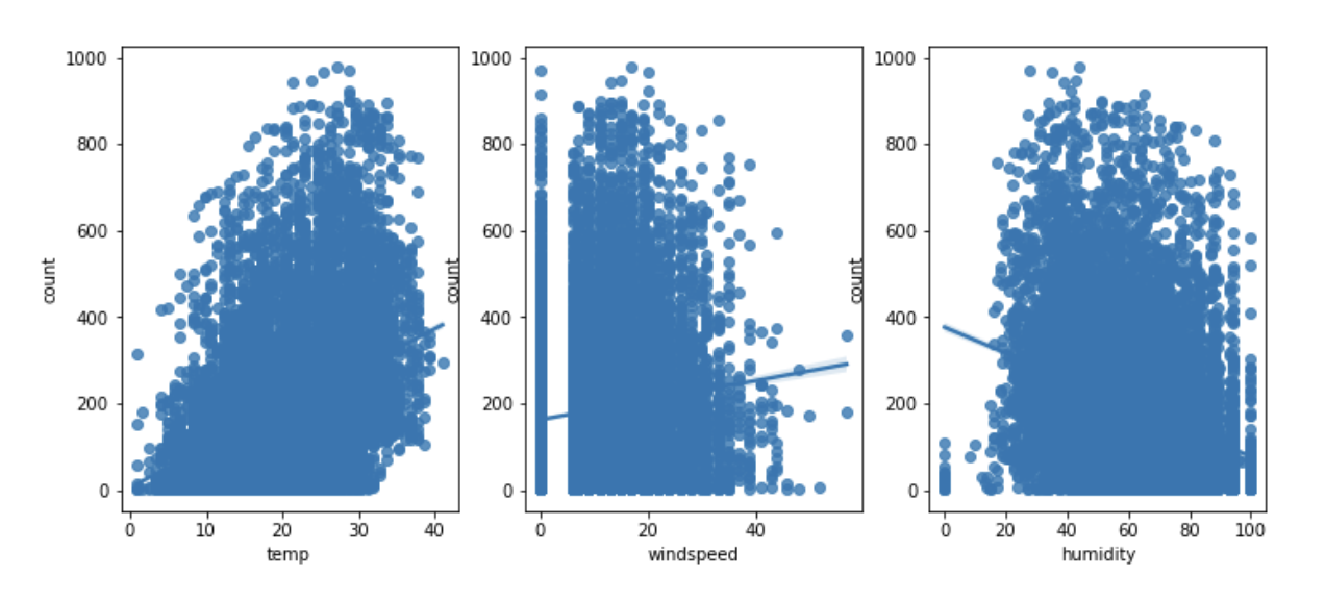
\includegraphics[scale=0.4,width=1.0\textwidth,height=0.4\textwidth]{graphics/img/scatterplot.eps}}
          \caption{Scatter Plot}\label{fig:Scatter Plot}
        \end{figure}
        \end{slide}
        %%
        %%==========================================================================================
    

  \begin{slide}[toc=,bm=]{ Correlation Matrix }
    \begin{itemize}
      \item  Heatmap of the correlation matrix between count and [temp, atemp, humidity, windspeed, casual, registered].
    \end{itemize}
    \begin{figure}
      \centering
      %\selectcolormodel{rgb}
      \centerline{\includegraphics[scale=0.4,width=0.8\textwidth,height=0.4\textwidth]{graphics/img/heatmap.eps}}
      \caption{Heatmap}\label{fig:Heatmap}
    \end{figure}
    \end{slide}
    %%
    %%==========================================================================================

\begin{slide}[toc=,bm=]{Feature Engineering}
Based on the above heatmap, we can see that some of the features have no relation with the response variable. we can drop those columns.
\begin{itemize}
\item
\textcolor{orange} {humidity}, \textcolor{orange}{temp} are negatively correlated with count
\item
There is a strong correlation between \textcolor{orange} {temp} and \textcolor{orange} {atemp}, if both are included in the model, it will cause multicollinearity problems, so one of the features must be deleted. We remove the atemp feature because it has a weaker correlation with count than temp.
\item
\textcolor{orange} {Casual}, \textcolor{orange}{Registered} are not considered and removed during model building 
\item
\textcolor{orange} {humidity}, \textcolor{orange}{temp} and \textcolor{orange} {windspeed} features are considered during future modelling
\item 
fill in the zero values in the windspeed feature: usage is high when the wind speed is 0, which may be caused by null filling. Therefore, a random forest model is used here to fill in the zero values. 
\end{itemize}

%%==========================================================================================

\end{slide}



%%==========================================================================================
%%c

\begin{slide}[toc=,bm=]{ Skewness in Data Distribution}

  \begin{itemize}
  \item From the histogram plot, we can say that count data is skewed (concentrated on the one side) and the data is not equally distributed.
  \item Solution is to log-transform the count variable after removing outlier data points.
  \end{itemize}
  \begin{figure}
    \centering
    %\selectcolormodel{rgb}
    \centerline{\includegraphics[scale=0.4,width=1.0\textwidth,height=0.4\textwidth]{graphics/img/skewness_before.eps}}
    \caption{Count distribution before logarithmic transformation}\label{fig:Count distribution before logarithmic transformation}
  \end{figure}
  \end{slide}
  %%
  %%==========================================================================================

  \begin{slide}[toc=,bm=]{ Solution to Skewness in Data Distribution}

    \begin{itemize}
    \item Solution is to log-transform the count variable after removing outlier data points.
    \end{itemize}
    \begin{figure}
      \centering
      %\selectcolormodel{rgb}
      \centerline{\includegraphics[scale=0.4,width=1.0\textwidth,height=0.4\textwidth]{graphics/img/skewness_after.eps}}
      \caption{Count distribution after logarithmic transformation}\label{fig:Count distribution after logarithmic transformation}
    \end{figure}
    \end{slide}
    %%
    %%==========================================================================================

    
\section{Predictive Modelling}


%%==========================================================================================
%%
\begin{slide}[toc=,bm=]{Data Preparation}
  
  \begin{itemize}
  \item Split the dataset into train set and test set
  \item Train Data size : 0.7
  \item Test Data size : 0.3
  
  \end{itemize}
  
  \end{slide}
  
  %%==========================================================================================

\begin{slide}[toc=,bm=]{Predictions with linear Model}
%Step One - Group Feature Extraction}
\begin{itemize}
\item Linear Regression
\item Ridge Regression
\item Lasso Regression
\item Logistic Regression
\item ElasticNet

\end{itemize}

\end{slide}

%%==========================================================================================
%%
\begin{slide}[toc=,bm=]{Predictions with Ensemble learning Models}
%Step Two - Outlying Degree Scoring
\begin{itemize}
  \item Bagging Regressor
  \item Random Forest Regressor
  \item Gradient Boosting Regressor
  \item AdaBoost Regressor
  
  \end{itemize}

\end{slide}
%%
%%==========================================================================================



\section{Evaluation Results}


%%==========================================================================================
%%
\begin{slide}[toc=,bm=]{Evaluation}

\begin{center}
\begin{itemize}

\item Evaluation Indicators: root mean square error is required (Root Mean Squared Logarithmic Error, RMSLE) to evaluate the quality of the model. 
\smallskip

{$$ RMSLE = \sqrt{\frac{1}{n} \sum_{i=1}^n [\log(p_i + 1) - \log(a_i + 1)]^2} $$}
Among them, $n$ is the number of samples in the test set, $p_i$ is the test value, and $a_i$ is the actual value. The smaller the root mean square error, the better the fitting effect of the data, and the closer the test value is to the actual value.
\end{itemize}
\end{center}

\end{slide}
%%
%%==========================================================================================


\begin{slide}[toc=,bm=]{Model Evaluation Results}

\begin{table}[tb]
\setlength{\abovecaptionskip}{0pt}
\setlength{\belowcaptionskip}{10pt}
\centering
\caption{Model Evaluation Results}

\begin{tabular}{ c | c | c | c }
\toprule
  % after \\: \hline or \cline{col1-col2} \cline{col3-col4} ...
  Model     & Accuracy      \\
\midrule
Random Forest Regression        & 0.376319   \\
Bagging Regression              & 0.395248    \\
GBRT                            & 0.430378   \\
AdaBoost Regression             & 0.703528   \\ 
Ridge Regression                & 1.045335   \\
Lasso Regression                & 1.045453 \\
ElasticNet Regression           & 1.045489 \\
Linear Regression               & 1.046341 \\
Logistic Regression             & 1.131105 \\
\bottomrule
\end{tabular}
\end{table}

%%==========================================================================================


\end{slide}
%%
%%==========================================================================================


\section{Conclusion}

%%==========================================================================================
%%
\begin{slide}[toc=,bm=]{Conclusion}
\begin{itemize}
\item
\smallskip
Basic modelling of the data

\item
\smallskip
Results can be further enhanced

\end{itemize}

\end{slide}
%%
%%==========================================================================================

%
\begin{slide}[toc=,bm=]{Questions?}
\begin{center}
\begin{figure}
    \animategraphics[autoplay, loop, height=0.4\textheight]{5}{./graphics//gif//question//q_}{1}{30}
\end{figure}
\end{center}
\end{slide}
%%
%%==========================================================================================


%%==========================================================================================
% TODO: Contact Page
\begin{wideslide}[toc=,bm=]{Contact Information}
\centering
\vspace{\stretch{1}}
\twocolumn[
lcolwidth=0.35\linewidth,
rcolwidth=0.65\linewidth
]
{
% \centerline{\includegraphics[scale=.2]{tulip-logo.eps}}
}
{
\vspace{\stretch{1}}
Pratikshya Parajuli\\
Ministry of Finance\\
Government of Nepal
\begin{description}
 \item[\textcolor{orange}{\faEnvelope}] \href{mailto:gangli@tulip.org.au}
 {\textsc{\footnotesize{misspratikshya@gmail.com}}}
\end{description}
}
\vspace{\stretch{1}}
\end{wideslide}

\end{document}

\endinput
